\subsection{Coupled Cluster Doubles with Realistic Nuclear Interactions}

Now, we can move on from analyzing pure neutron matter and instead turn our attention to symmetric nuclear matter (SNM), which comprises an equivalent number of protons and neutrons. We will continue to use the chiral NNLO potentials. Here all SNM systems will be calculated using 132 nucleons (66 protons and 66 neutrons) since these results will be similar to the energies at the TDL \cite{Ref9}.   Furthermore, the immense computational costs of SNM calculations also prohibit studies and higher particle numbers. Compared to a PNM calculation, an SNM calculation will need to double the number of single-particle states to accommodate double the number of particles. It will need approximately three times the computational time and resources. However, it is essential to perform calculations of SNM in addition to PNM even at the higher computational costs because the addition of protons into the system causes different correlations in the system, leading to a correlation energy that converges slower with respect to the number of single-particle states. Thus SNM should be a more challenging system for the SRE method and will genuinely test its predictive abilities.
Additionally, as we think about moving towards calculations of finite nuclei in future works, accurate calculations of both PNM and SNM are essential for these studies. Fig. \ref{fig:pnm_and_snm} compares the CCD correlation energies per nucleon for PNM (red) and SNM (blue). We can see that the SNM correlation energies are significantly larger than the PNM ones.



\begin{figure}
    \centering
    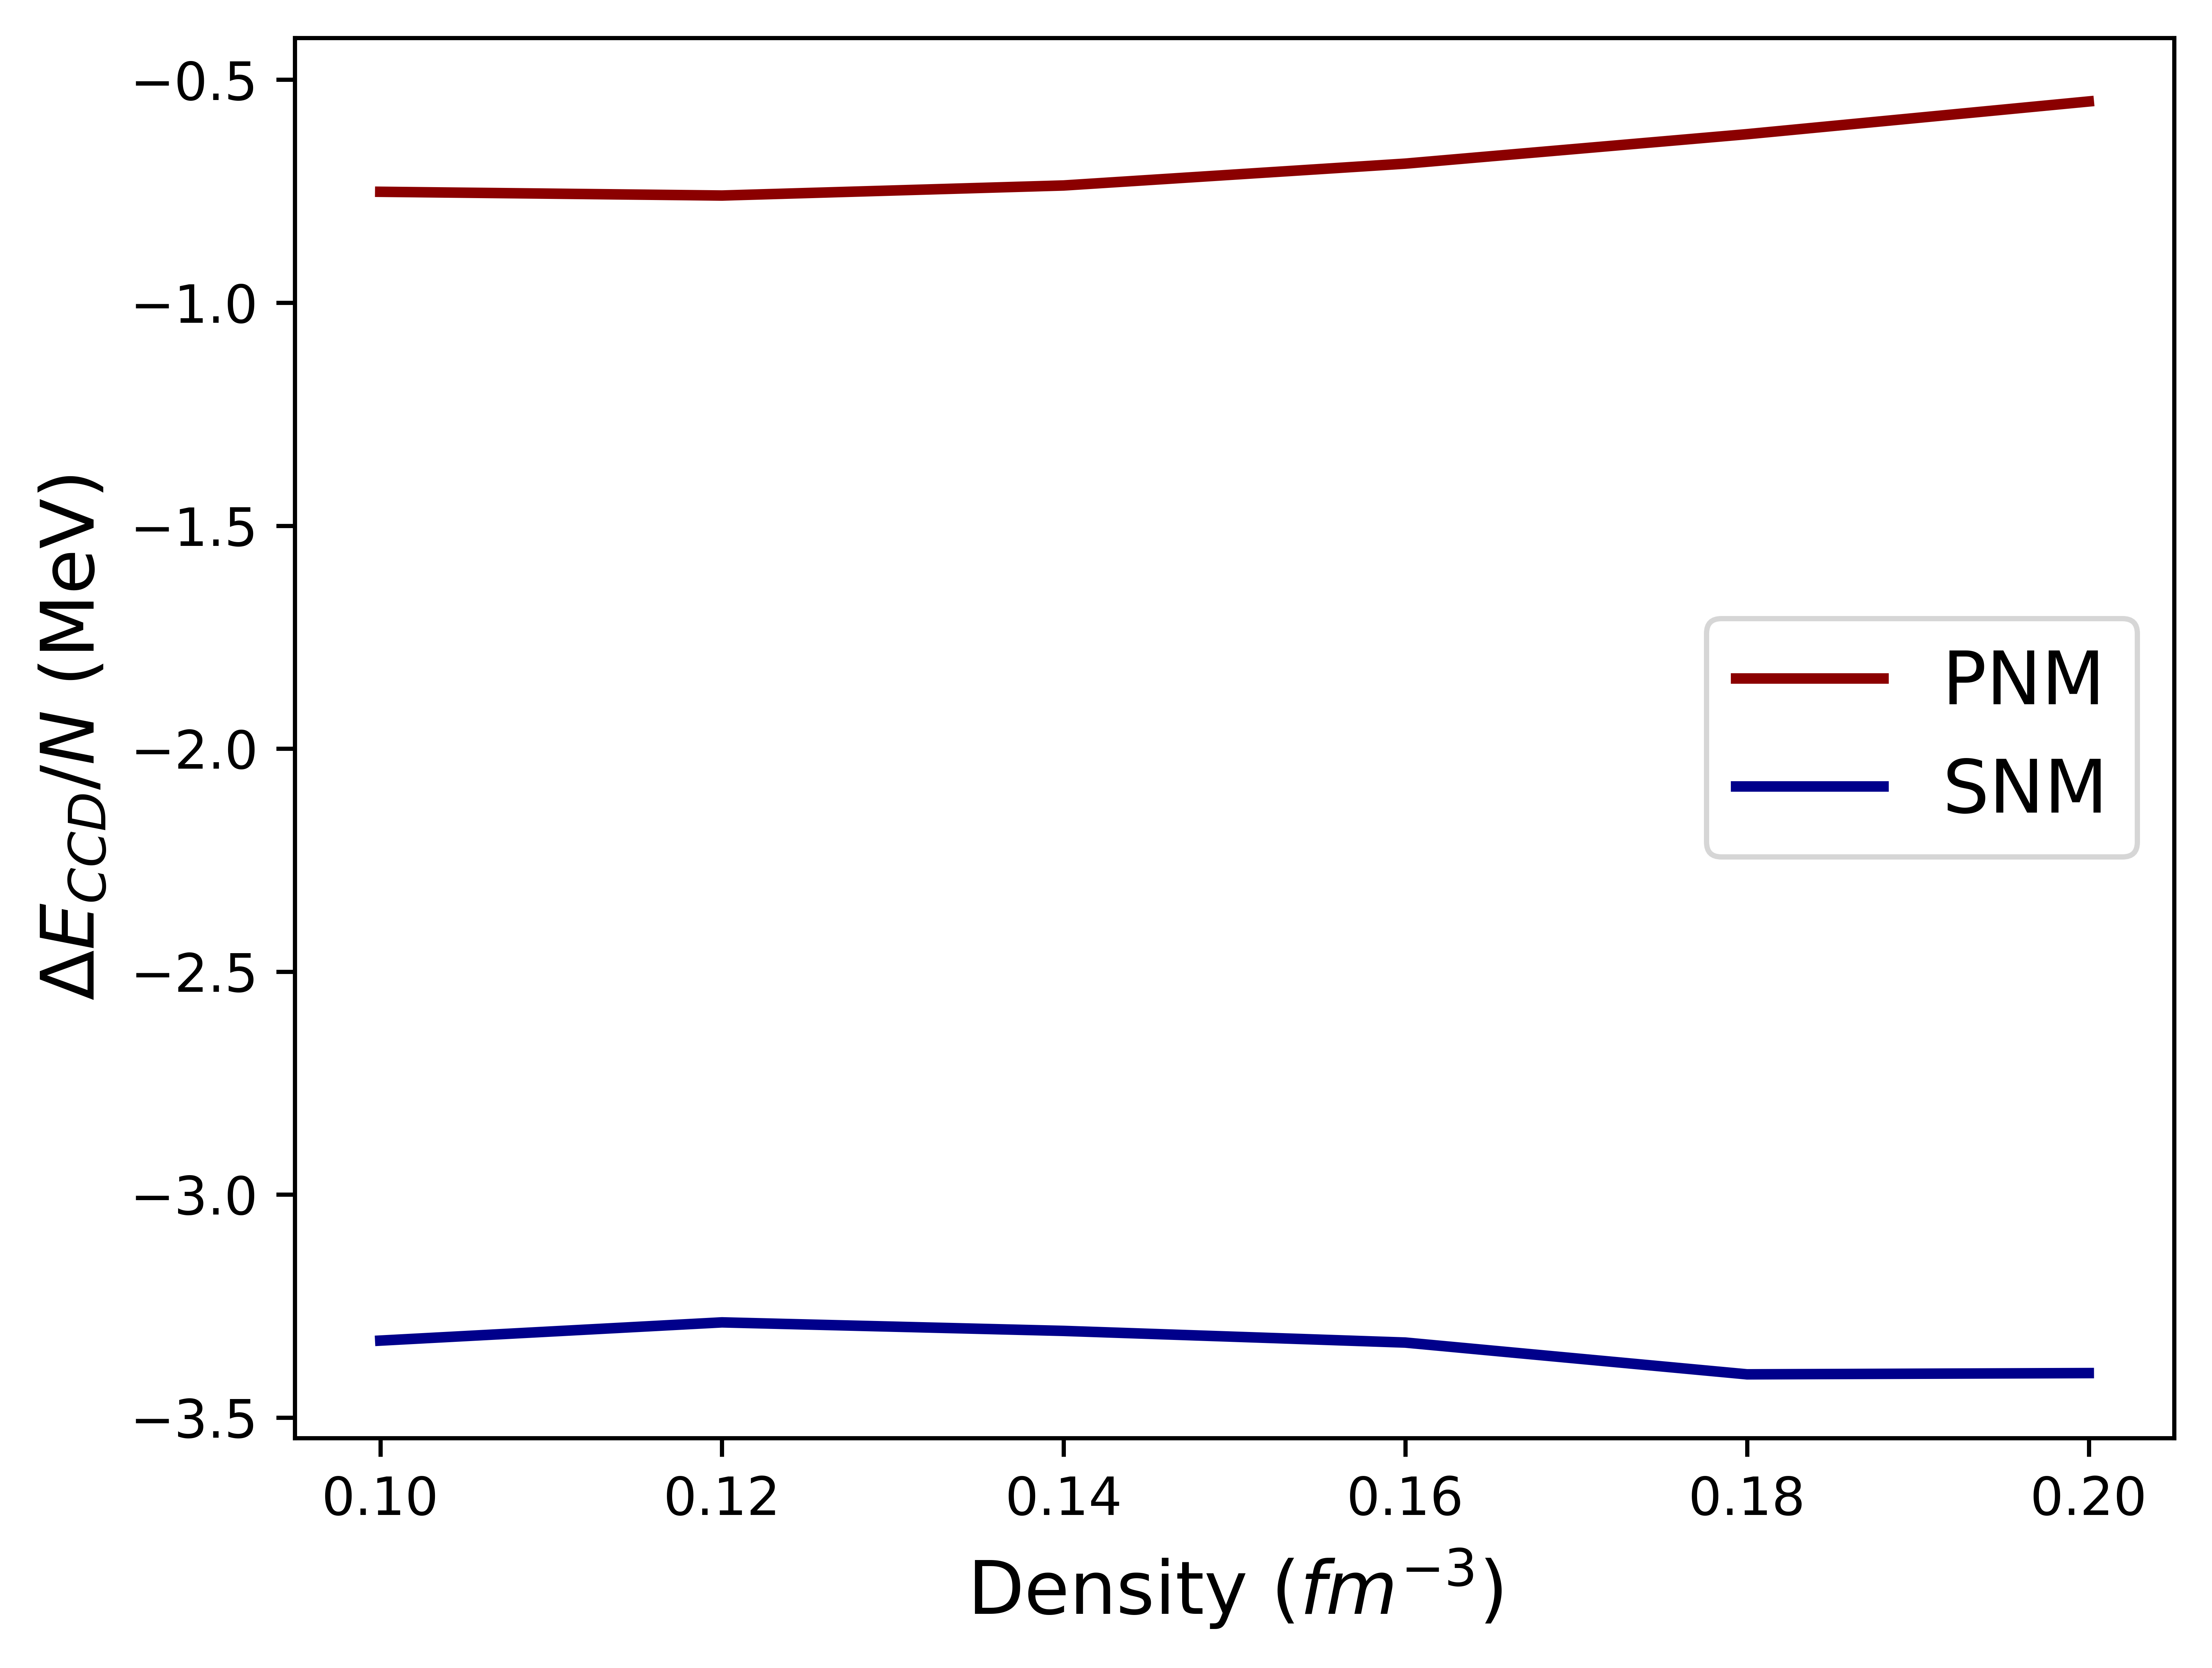
\includegraphics[scale=0.75]{Images/Chapter8/pnm_and_snm.png}
    \caption{The CCD correlation energies for PNM (red) and SNM (blue) for densities around nuclear matter and with a chiral NNLO potential.}
    \label{fig:pnm_and_snm}
\end{figure}

The CCD data set for SNM was generated using a supercomputer available through Michigan State University's Institute for Cyber-Enabled Research (ICER) using Intel Xeon processors, which have a clock speed of 2.4 GHz. For the MPI parallelization, 24 nodes were used. It takes, on average, 26.07 node hours to generate a converged CCD energy for a PNM system (at M = 1,478). However, since SNM is a more challenging case, and the number of single-particle states doubles, it takes, on average, 84.12 node hours to perform a converged CCD correlation energy calculation for SNM at M = 2,956. This means the computational resources needed for an SNM calculation are more significant than those needed for a PNM calculation by about a factor of three.

\begin{figure}
    \centering
    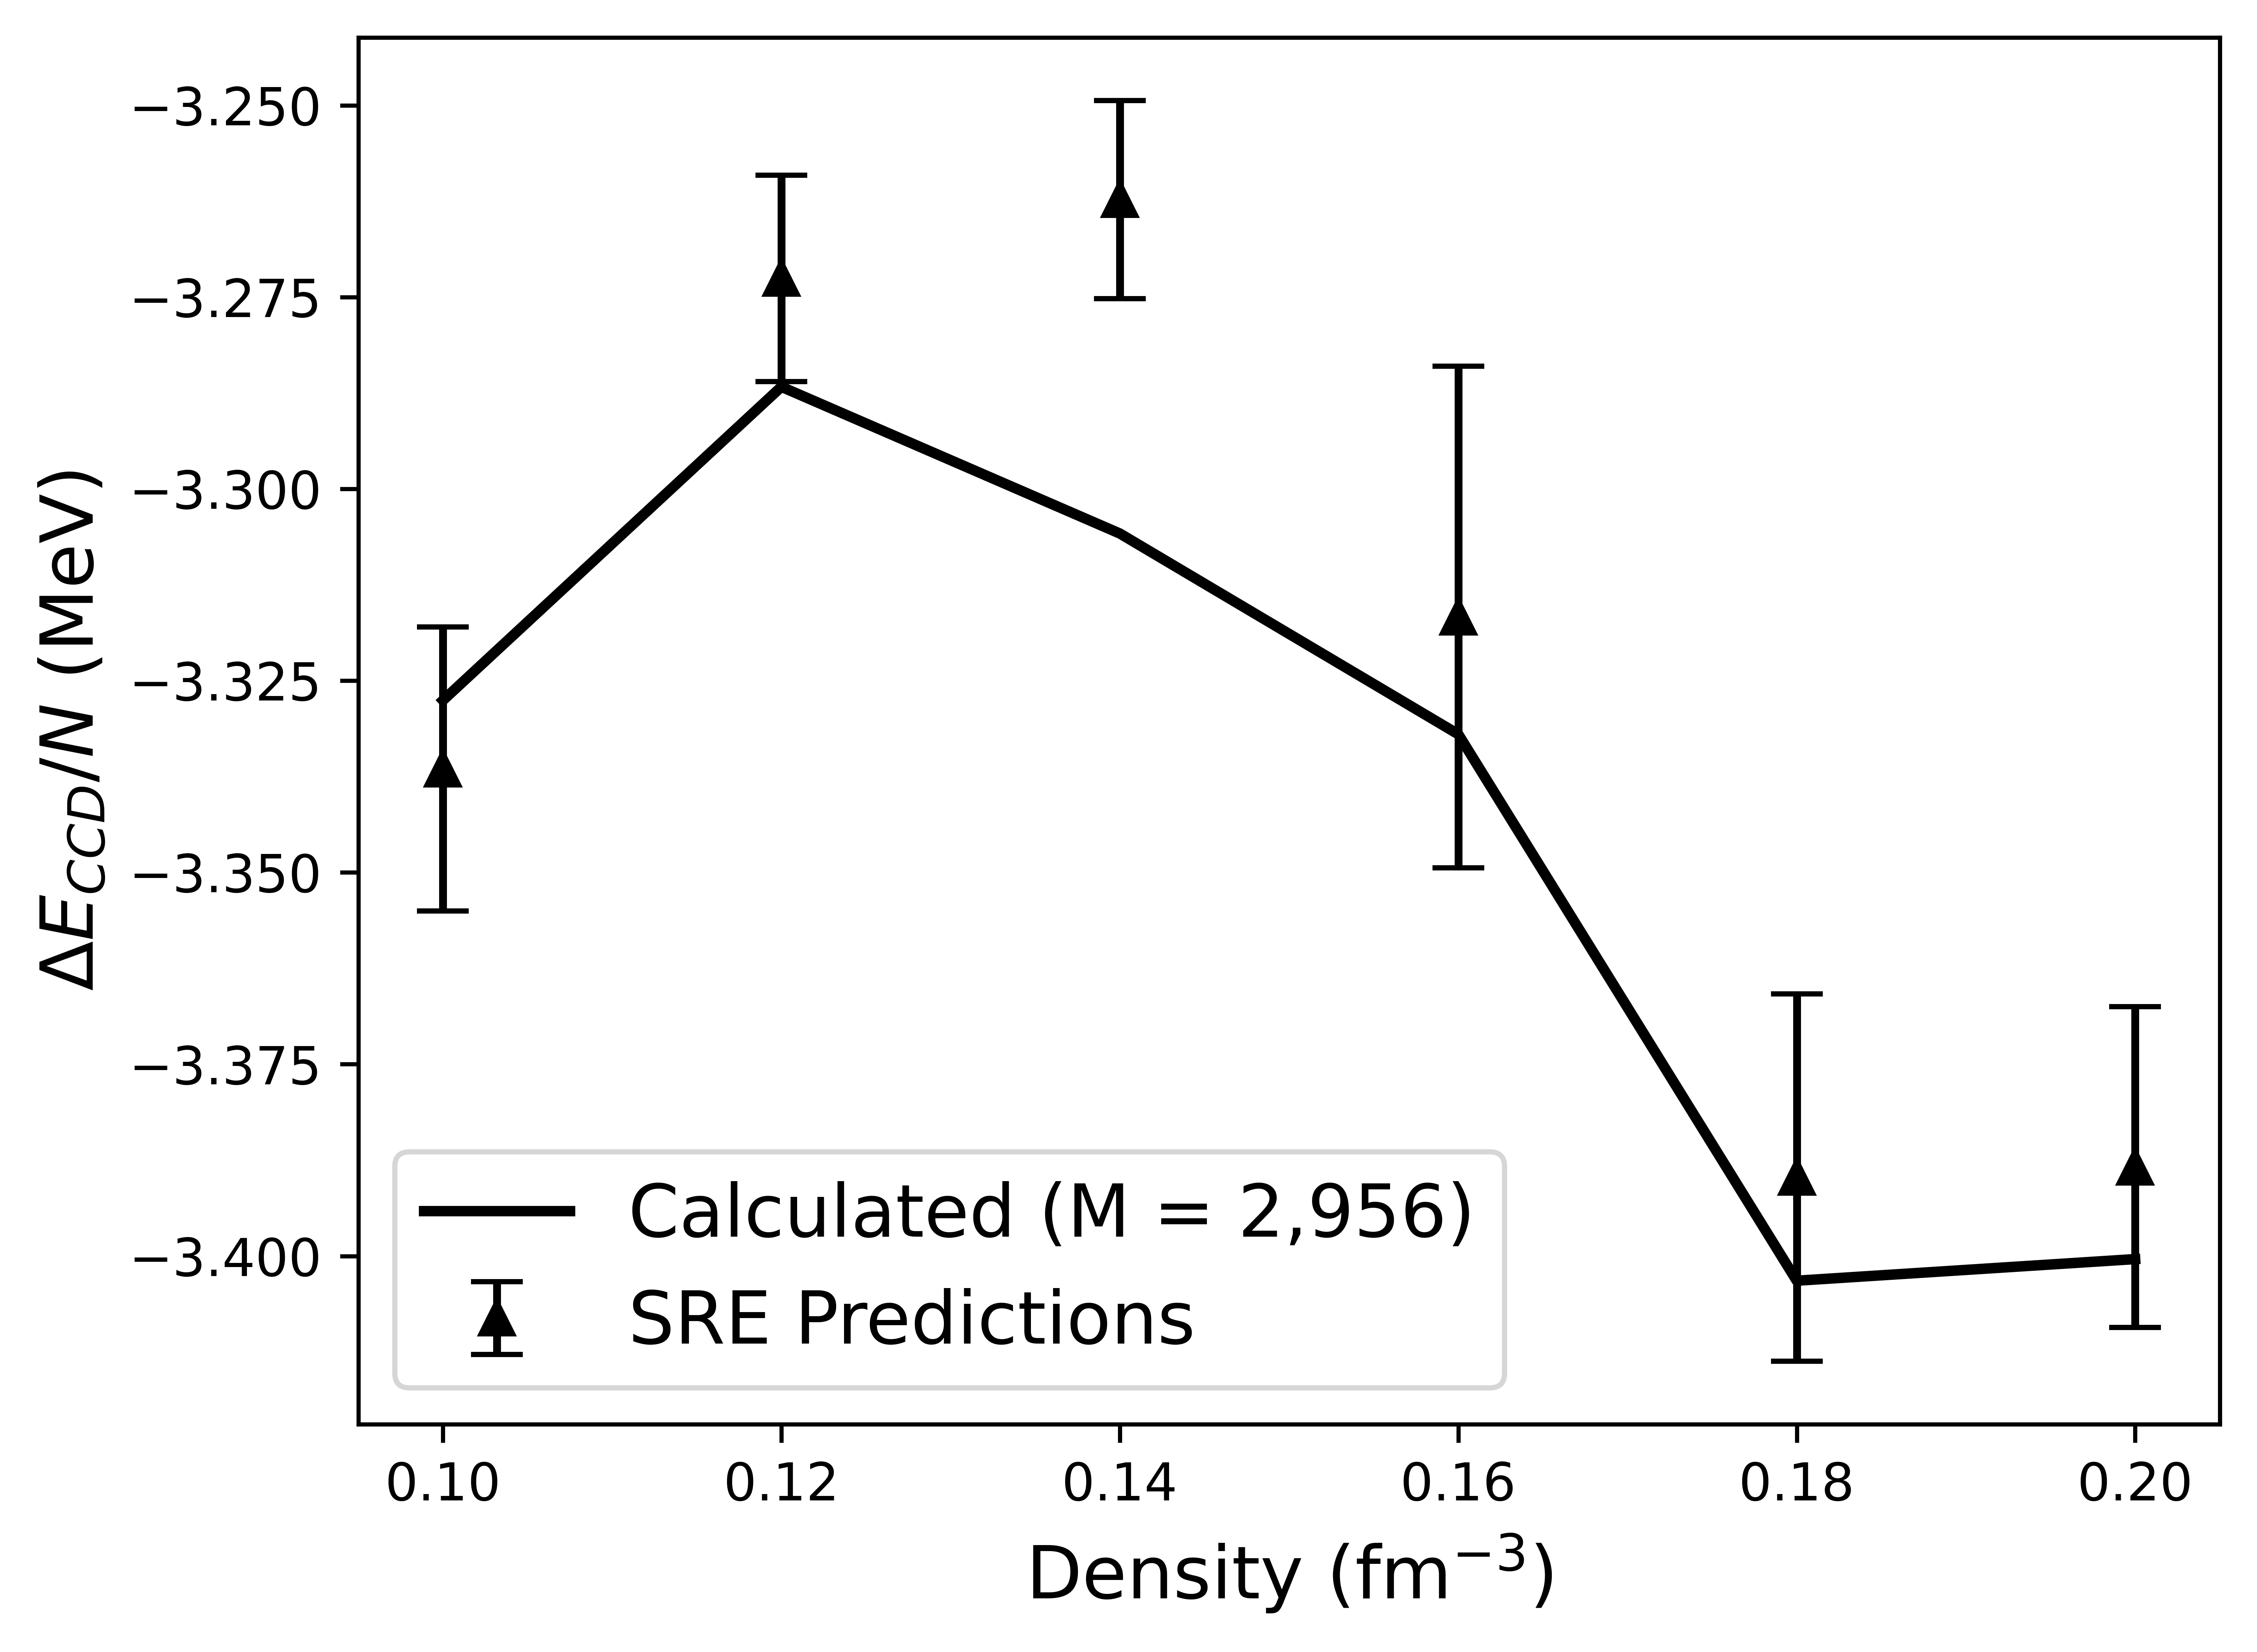
\includegraphics[scale=0.75]{Images/Chapter8/FinalReport3b-3.png}
    \caption{The CCD correlation energies for SNM calculated fully at M = 2,956 (solid line) and using the SRE method to predict them (triangular marker).  The average percent error of this graph is 0.54$\%$ and the time savings of using SRE over performing the full calculations is 6.48 node days.}
    \label{fig:snm_ccd}
\end{figure}

The SRE predictions in Fig. \ref{fig:snm_ccd} were generated using seven training points from M = 324 to M = 1,004. The SRE sequence length is used as three since there are more training data points here compared to the PNM case. In addition, the SNM CCD energy has a slower convergence than the PNM energies, leading to the use of more training data.

When predicting the CCD correlation energies using the SRE method, the average percent error between the predictions and the complete calculations at M = 2,956 is 0.54$\%$. This is compared to the average percent error between the calculations at M = 2,956 and M = 1,004 (the largest training data point) of 9.52$\%$. Thus the SRE provides a much more accurate method than truncating the calculations at the level of the training data. Furthermore, it takes 504.77 node hours to compute all six data points shown in Fig. \ref{fig:snm_ccd} at M = 2,956 but only 349.17 node hours to generate the training data needed by the SRE algorithm to predict all 6 points. This leads to a computational time savings of 155.61 node hours or 6.48 \textit{node days}. Thus the SRE method can accurately recreate the CCD correlation energies of an SNM system with significant time savings.